\documentclass[14pt]{article}
\usepackage[T1,T2A]{fontenc}
\usepackage[utf8]{inputenc}
\usepackage[english,russian]{babel}
\usepackage{graphicx}
\usepackage{amsmath}
\usepackage{float}
\graphicspath {{img/}}

\title{\textbf{Лабораторная работа №6\\<<Помехоустойчивое кодирование. Код Хэмминга>>}}
\author{Матяш А.А., ККСО-01-19}
\date{}
\addtolength{\topmargin}{-3cm}
\addtolength{\textheight}{3cm}
\begin{document}
\maketitle
\thispagestyle{empty}
\textbf{Цель работы:}  ознакомление с принципами помехоустойчивого кодирования и приобретение практических навыков моделирования работы кодеров и декодеров. 

\section{Задание №1: формирование бита чётности}

\subsection{Формирование бита чётности}
Сформировать бит чётности (бит паритета) для заданного байта передаваемых данных. Исходными данными является последовательность 10111001 (14-й вариант).

Паритетный бит $k$ для n-битного двоичного слова $b_n \ldots b_2 b_1$ вычисляется по формуле:
$$
k=b_n \oplus \ldots \oplus b_2 \oplus b_1
$$

Таким образом, число единиц в последовательности будет всегда чётным. Для нашего примера получим выражение:
$$
k= 1 \oplus 0 \oplus 1\oplus 1\oplus 1\oplus 0\oplus 0\oplus 1 = 1
$$
Тогда $k=1$, кодовая комбинация будет равна: 101110011.

\newpage

\section{Задание №2: Исследование помехоустойчивого кода с формированием бита чётности}

\subsection{Исходные данные для задания}

\begin{table}[h]
\begin{tabular}{|c|c|c|c|c|}
\hline
\begin{tabular}[c]{@{}c@{}}Информационные биты \\ S4S3S2S1\end{tabular} &
  \begin{tabular}[c]{@{}c@{}}Помехи \\ S8S7S6S5\end{tabular} &
  \begin{tabular}[c]{@{}c@{}}Помехи \\ S8S7S6S5\end{tabular} &
  \begin{tabular}[c]{@{}c@{}}Помехи \\ S8S7S6S5\end{tabular} &
  \begin{tabular}[c]{@{}c@{}}Помехи \\ S8S7S6S5\end{tabular} \\ \hline
1101 &
  0000 &
  0100 &
  0110 &
  0111 \\ \hline
\end{tabular}
\end{table}

\begin{center}
    Таблица 1 - Исходные данные для задания №2
\end{center}

\subsection{ Перечень элементов, использованных в схемах, с их краткими характеристиками}
\begin{itemize}
    \item[-] XOR5 
    \item[-] XOR4
    \item[-] XOR2 - 4 шт.
    \item[-] Цифровой источник питания
    \item[-] Ключ - 8 шт.
    \item[-] Индикатор - 2 шт.
\end{itemize}
\subsection{Схема для моделирования процесса передачи информации по каналу связи}

\begin{center}
    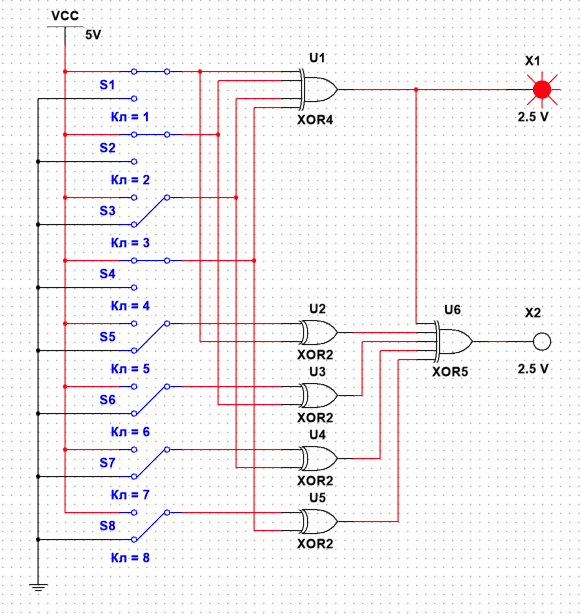
\includegraphics[width=1\linewidth]{img/scheme1.png}
    Рис. 1 - Схема для исследования кода с формированием бита чётности
\end{center}


\indentСветодиод X1 показывает значение бита четности. Если датчик горит красным, значит бит четности равен 1, если не горит — 0. Если светодиод X2 не горит, то считается, что нечетного числа ошибок нет.\\
\indentЗаполним таблицу (см. Таблица 1). Например, на схеме показаны положения переключателей при битах помех равному 0000. Тогда в столбец X2 запишем значение 0. Сделаем также и для остальных случаев.\\
\begin{table}[h]
\begin{tabular}{|c|c|c|c|c|}
\hline
S8 & S7 & S6 & S5 & X2 \\ \hline
0  & 0  & 0  & 0  & 0  \\ \hline
0  & 1  & 0  & 0  & 1  \\ \hline
0  & 1  & 1  & 0  & 0  \\ \hline
0  & 1  & 1  & 1  & 1  \\ \hline
\end{tabular}
\end{table}

\indentПри первом моделирование с битам помех 0000, очевидно, ошибок нет.\\
\indentПри втором моделирование с битами помех 0100 возникает одна ошибка и контрольный бит четности помогает поймать ошибку, сигнализируя что в выходящей и выходящей последовательности четность разная.\\
\indentПри третьем моделирование с битами помех 1100 ошибка не возникает.
\indentПри четвертом моделирование с битами помех 0111 теперь возникает ошибка, и, соответственно, четность нарушена, о чем сигнализирует X2
\section{Задание №3: Исправление ошибки с помощью кода Хэмминга}
Расчётным путём, точнее вручную, определим, в каком разряде кода Хэмминга произошло искажение. 
\subsection{Исходные данные для задания}
\begin{center}
\begin{table}[h]
\begin{tabular}{|c|c|c|c|c|c|c|c|c|c|c|c|}
\hline
\textit{i8} & \textit{i7} & \textit{i6} & \textit{i5} & \textit{k4} & \textit{i4} & \textit{i3} & \textit{i2} & \textit{k3} & \textit{i1} & \textit{k2} & \textit{k1} \\ \hline
1           & 0           & 1           & 0           & 0           & 1           & 1           & 1           & 1           & 1           & 0           & 0           \\ \hline
\end{tabular}
\end{table}
        Таблица 2 - Исходные данные для задания №3.
\end{center}

\subsection{Процесс вычисления искажённого бита}
Найдём значения k-х битов на приеме:

$k'_1 = i_3 \oplus i_5 \oplus i_7 \oplus i_9 \oplus i_{11} = 1 \oplus 1 \oplus 1 \oplus 0 \oplus 0 = 1$ \\

$k'_2 = i_3 \oplus i_6 \oplus i_7 \oplus i_{10} \oplus i_{11} = 1 \oplus 1 \oplus 1 \oplus 1 \oplus 0 = 0$ \\

$k'_3 = i_5 \oplus i_6 \oplus i_7 \oplus i_{12} = 1 \oplus 1 \oplus 1 \oplus 1 = 0$ \\

$k'_4 = i_9 \oplus i_{10} \oplus i_{11} \oplus i_{12}= 0 \oplus 1 \oplus 0 \oplus 1 = 0$ \\

k-е биты на передающей принимающей стороне отличаются, что
свидетельствует о наличии ошибки.\\

Определим синдром $S = S_4 S_3 S_2 S_1$:\\

$S_1 = k_1 \oplus k'_1 = 0 \oplus 1 = 1$\\

$S_2 = k_2 \oplus k'_2 = 0 \oplus 0 = 0$\\

$S_3 = k_3 \oplus k'_3 = 1 \oplus 0 = 1$\\

$S_4 = k_4 \oplus k'_4 = 0 \oplus 0 = 0$\\

$S = 0101_2 = 5_{10} =>$ 5-й бит искажен. Корректный код будет иметь вид:

\begin{table}[h]
\begin{tabular}{|c|c|c|c|c|c|c|c|c|c|c|c|}
\hline
\textit{i8} & \textit{i7} & \textit{i6} & \textit{i5} & \textit{k4} & \textit{i4} & \textit{i3} & \textit{i2} & \textit{k3} & \textit{i1} & \textit{k2} & \textit{k1} \\ \hline
1           & 0           & 1           & 0           & 0           & 1           & 1           & 0           & 1           & 1           & 0           & 0           \\ \hline
\end{tabular}
\end{table}

\section{Задание №4: Моделирование работы кода Хэмминга}
\subsection{Исходные данные для задания}
Исходные данные приведены в таблице 2.
\subsection{Перечень элементов, использованных в схемах, с их краткими характеристиками.}
\begin{itemize}
    \item [-] XOR5 - 4 шт.
    \item [-] XOR4 - 4 шт.
    \item [-] XOR2 - 16 шт.
    \item [-] Цифровой источник питания
    \item [-] Генератор слов
    \item [-] Ключ - 8 шт.
    \item [-] Индикатор - 12 шт.
\end{itemize}
\subsection{Схема для исследования работы кода Хэмминга}
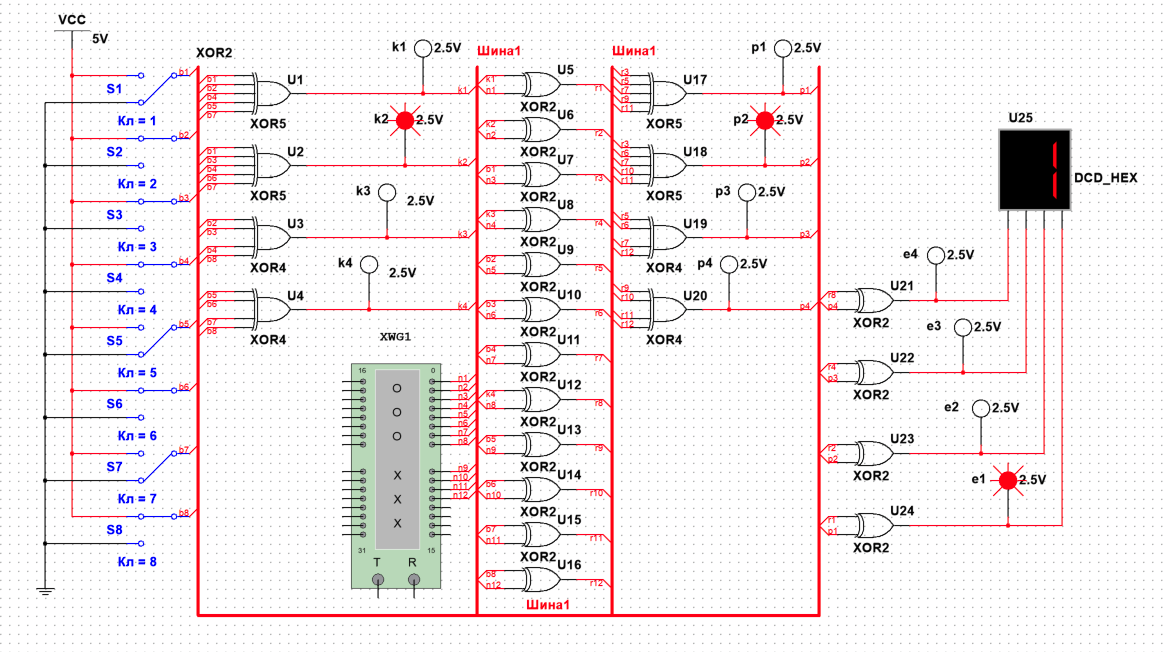
\includegraphics[width=1\linewidth]{img/scheme2.png}
\begin{center}
        Рис 6 - Схема моделирования работы кода Хэмминга в системе передачи информации.
\end{center}

\subsection{Результаты расчётов}
Ниже представлена таблица помех и показаний схемы моделирования работы кода Хэмминга:

\begin{table}[H]
    \resizebox{\textwidth}{!}{
    \begin{tabular}{llll}
    \hline
    \multicolumn{1}{|c|}{В каком бите искажение}     & \multicolumn{1}{c|}{Значения контрольных битов на приёмнике} & \multicolumn{1}{c|}{Синдром} & \multicolumn{1}{c|}{HEX}\\ \hline
    \multicolumn{1}{|c|}{$k_1$}                       &\multicolumn{1}{|c|}{0010}                        &\multicolumn{1}{|c|}{0001}            &\multicolumn{1}{|c|}{1}            \\ \hline
    \multicolumn{1}{|c|}{$k_2$}                       &\multicolumn{1}{|c|}{0010}                        &\multicolumn{1}{|c|}{0010}            &\multicolumn{1}{|c|}{2}            \\ \hline
    \multicolumn{1}{|c|}{$i_1$}                       &\multicolumn{1}{|c|}{1110}                        &\multicolumn{1}{|c|}{0011}            &\multicolumn{1}{|c|}{3}            \\ \hline
    \multicolumn{1}{|c|}{$k_3$}                       &\multicolumn{1}{|c|}{0010}                        &\multicolumn{1}{|c|}{0100}            &\multicolumn{1}{|c|}{4}            \\ \hline
    \multicolumn{1}{|c|}{$i_2$}                       &\multicolumn{1}{|c|}{1000}                        &\multicolumn{1}{|c|}{0101}            &\multicolumn{1}{|c|}{5}            \\ \hline
    \multicolumn{1}{|c|}{$i_3$}                       &\multicolumn{1}{|c|}{0100}                        &\multicolumn{1}{|c|}{0110}            &\multicolumn{1}{|c|}{6}            \\ \hline
    \multicolumn{1}{|c|}{$k_4$}                       &\multicolumn{1}{|c|}{1100}                        &\multicolumn{1}{|c|}{0111}            &\multicolumn{1}{|c|}{7}            \\ \hline
    \multicolumn{1}{|c|}{$i_4$}                       &\multicolumn{1}{|c|}{0010}                        &\multicolumn{1}{|c|}{1000}            &\multicolumn{1}{|c|}{8}            \\ \hline
    \multicolumn{1}{|c|}{$i_5$}                       &\multicolumn{1}{|c|}{1010}                        &\multicolumn{1}{|c|}{1001}            &\multicolumn{1}{|c|}{9}            \\ \hline
    \multicolumn{1}{|c|}{$i_6$}                       &\multicolumn{1}{|c|}{0111}                        &\multicolumn{1}{|c|}{1010}            &\multicolumn{1}{|c|}{A}            \\ \hline
    \multicolumn{1}{|c|}{$i_7$}                       &\multicolumn{1}{|c|}{1111}                        &\multicolumn{1}{|c|}{1011}            &\multicolumn{1}{|c|}{B}            \\ \hline
    \multicolumn{1}{|c|}{$i_8$}                       &\multicolumn{1}{|c|}{0001}                        &\multicolumn{1}{|c|}{1100}            &\multicolumn{1}{|c|}{C}            \\ \hline
    \end{tabular}
    }
    \end{table} \\

\textbf{Вывод:} В ходе работы были изучены теоретические аспекты помехоустойчивого кодирования, а также приобретены практические навыки моделирования работы кода Хэмминга.

\end{document}
